\documentclass[aspectratio=43]{beamer}

\usepackage{amsmath}
\usepackage{amssymb}
\usepackage{tikz}

\usetheme{Madrid}
\usecolortheme{default}

\setbeamertemplate{navigation symbols}{}

\setbeamertemplate{footline}{}

\title{}
\author{}
\date{}

\begin{document}

\begin{frame}
    \frametitle{Boolean functions}
    \begin{block}{Problem}
        How many Boolean functions in $k$ variables are there?
    \end{block}

    \begin{block}{Solution}
        Each of the $k$ input bits can take value 0 or 1. There are $2^k$ possible input binary strings. A Boolean function can send each of them to either 0 or 1. So the total number of possibilities is $2^{2^k}$.
    \end{block}

    \begin{block}{Exercise}
        Count microchips with $k$ binary inputs and $\ell$ binary outputs. Two microchips are considered identical if they compute the same function \{binary strings of length $k$\} $\rightarrow$ \{binary strings of length $\ell$\}.

        For $\ell = 1$, you should recover the previous answer.
    \end{block}
\end{frame}

\begin{frame}
    \frametitle{Problem-solving challenges}
    In past years, many students ended up dropping out of Math 465.
    Why? Much of the content is quite elementary.

    However, many problems are ``one of a kind,'' with no off-the-shelf algorithmic solution.
    The first two quizzes will give you some idea of where you stand.

    How do I prepare for quizzes/exams/homework?
    Use problems in the textbooks to practice!
    Also, come to office hours.

    Questions?
\end{frame}

\begin{frame}
    \frametitle{Basic counting principles [Chapter 3]}
    First half of the course: \textit{enumerative combinatorics}.

    We will study the basic techniques of \textit{counting}, or \textit{enumeration}.

    \begin{block}{Two versions of counting}
        (1) Counting concrete objects;

        (2) Counting choices/possibilities.
    \end{block}

    \begin{block}{Examples}
        (1) counting beer bottles in a party store;

        (2) buying plane tickets for a given itinerary.
    \end{block}
\end{frame}

\begin{frame}
    \frametitle{Subsets and binary strings}
    \begin{block}{Theorem}
        A $k$-element set has $2^k$ subsets.
    \end{block}

    \[
        \boxed{k=3} \quad \emptyset \quad \{A\} \quad \{B\} \quad \{C\} \quad \{A,B\} \quad \{A,C\} \quad \{B,C\} \quad \{A,B,C\}
    \]

    \begin{block}{Proof}
        The subsets of a $k$-element set are encoded by binary strings of length $k$, i.e., by $k$-letter words in a 2-letter alphabet:
        \[
            \emptyset \quad \{A\} \quad \{B\} \quad \{C\} \quad \{A,B\} \quad \{A,C\} \quad \{B,C\} \quad \{A,B,C\}
        \]
        \[
            000 \quad 100 \quad 010 \quad 001 \quad 110 \quad 101 \quad 011 \quad 111
        \]
        The number of such words is $2^k$.
    \end{block}
\end{frame}

\begin{frame}
    \frametitle{Counting words}
    An \textit{alphabet} is a finite set of symbols (letters).

    A \textit{word} in an alphabet is a string (i.e., finite sequence) of letters.

    \begin{block}{Theorem}
        The number of $k$-letter words in an $n$-letter alphabet is $n^k$.
    \end{block}

    \[
        \begin{array}{ll}
            k=2 \\
            n=3
        \end{array}
        \quad
        AA \quad AB \quad AC \quad BA \quad BB \quad BC \quad CA \quad CB \quad CC
    \]

    \[
        \begin{array}{ll}
            k=3 \\
            n=2
        \end{array}
        \quad
        AAA \quad AAB \quad ABA \quad ABB \quad BAA \quad BAB \quad BBA \quad BBB
    \]
\end{frame}

\begin{frame}
    \frametitle{Cyclic permutations}
    \begin{block}{Problem}
        How many ways are there to arrange $n$ distinct objects in a circle, up to rotation?

        Example: seating a party of $n$ people around a round table.
    \end{block}

    \begin{center}
        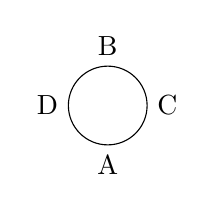
\begin{tikzpicture}
            \node[circle, draw, minimum size=1cm] (c1) {};
            \node[anchor=north] at (c1.south) {A};
            \node[anchor=east] at (c1.west) {D};
            \node[anchor=south] at (c1.north) {B};
            \node[anchor=west] at (c1.east) {C};
        \end{tikzpicture}
        \hspace{0.5cm}
        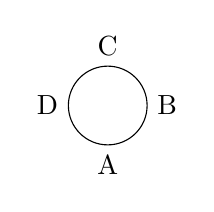
\begin{tikzpicture}
            \node[circle, draw, minimum size=1cm] (c2) {};
            \node[anchor=north] at (c2.south) {A};
            \node[anchor=east] at (c2.west) {D};
            \node[anchor=south] at (c2.north) {C};
            \node[anchor=west] at (c2.east) {B};
        \end{tikzpicture}
        \hspace{0.5cm}
        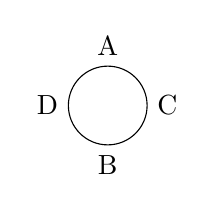
\begin{tikzpicture}
            \node[circle, draw, minimum size=1cm] (c3) {};
            \node[anchor=north] at (c3.south) {B};
            \node[anchor=east] at (c3.west) {D};
            \node[anchor=south] at (c3.north) {A};
            \node[anchor=west] at (c3.east) {C};
        \end{tikzpicture}
        \hspace{0.5cm}
        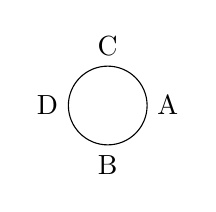
\begin{tikzpicture}
            \node[circle, draw, minimum size=1cm] (c4) {};
            \node[anchor=north] at (c4.south) {B};
            \node[anchor=east] at (c4.west) {D};
            \node[anchor=south] at (c4.north) {C};
            \node[anchor=west] at (c4.east) {A};
        \end{tikzpicture}
        \hspace{0.5cm}
        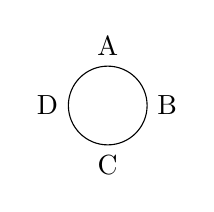
\begin{tikzpicture}
            \node[circle, draw, minimum size=1cm] (c5) {};
            \node[anchor=north] at (c5.south) {C};
            \node[anchor=east] at (c5.west) {D};
            \node[anchor=south] at (c5.north) {A};
            \node[anchor=west] at (c5.east) {B};
        \end{tikzpicture}
        \hspace{0.5cm}
        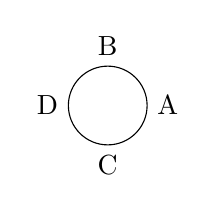
\begin{tikzpicture}
            \node[circle, draw, minimum size=1cm] (c6) {};
            \node[anchor=north] at (c6.south) {C};
            \node[anchor=east] at (c6.west) {D};
            \node[anchor=south] at (c6.north) {B};
            \node[anchor=west] at (c6.east) {A};
        \end{tikzpicture}
    \end{center}

    Answer: $(n-1)!$.

    \begin{block}{Exercise}
        Given $n$ beads of different colors, how many circular necklaces are there that use all of these beads?
    \end{block}
\end{frame}

\begin{frame}
    \frametitle{The Subtraction Principle}
    The Subtraction Principle is used in situations where it is more practical to count the objects of interest together with some other objects, and then subtract the number of those extra objects.

    \begin{block}{Problem}
        How many ways are there to place 5 people named Amy, Bernie, Cory, Donald, and Elizabeth on the stage so that Amy and Bernie are \textit{not} adjacent to each other?
    \end{block}

    \begin{block}{Solution}
        $5! - 4! \cdot 2 = 72$.
    \end{block}
\end{frame}

\begin{frame}
    \frametitle{The Division Principle}
    The Division Principle is used in situations where each object of interest is counted several times (a fixed number).

    \begin{block}{Problem}
        How many diagonals are there in a convex $n$-gon?
    \end{block}

    \begin{center}
        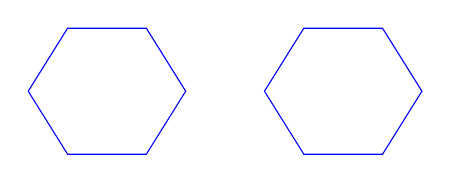
\begin{tikzpicture}
            \draw[blue] (0,0) -- (1,0) -- (1.5,0.8) -- (1,1.6) -- (0,1.6) -- (-0.5,0.8) -- cycle;
            \draw[blue] (3,0) -- (4,0) -- (4.5,0.8) -- (4,1.6) -- (3,1.6) -- (2.5,0.8) -- cycle;
            % Placeholder for illustrations
        \end{tikzpicture}
    \end{center}

    \begin{block}{Solution}
        For each of the $n$ vertices, there are $n-3$ diagonals connecting to it. Each diagonal is counted twice. Answer: $n(n-3)/2$.
    \end{block}
\end{frame}

\begin{frame}
    \frametitle{Course management}
    I am teaching Math 465 section 3 this Fall

    Location: East Hall B737

    Time: Tuesday and Thursday, 2:30-3:50 PM.

    The best way to communicate with me is by email.

    Most of the course management will occur on Canvas.

    Office hours will be conducted in my office, EH 3827:
    \begin{itemize}
        \item Tuesday/Thursdasy 3:50-5:20 PM
    \end{itemize}
\end{frame}

\begin{frame}
    \frametitle{Math 465: Introduction to Combinatorics}

    \begin{center}
        Andrew Sack

        \texttt{asack@umich.edu}
    \end{center}

    These slides will be posted on Canvas.
\end{frame}

\begin{frame}
    \frametitle{Permutations of subsets}
    \begin{block}{Problem}
        Given 34 people, how many ways are there for \textit{at most} 4 of them to wait in line?
    \end{block}

    \begin{block}{Solution}
        Let us divide the set of possibilities into \textit{cases}:
        \begin{itemize}
            \item The line has 0 people. There is 1 way this can happen.
            \item The line has 1 person. There are 34 ways this can happen.
            \item The line has 2 people. There are $34 \cdot 33 = 1122$ ways.
            \item The line has 3 people. There are $34 \cdot 33 \cdot 32 = 35904$ ways.
            \item The line has 4 people. There are $34 \cdot 33 \cdot 32 \cdot 31 = 1113024$ ways.
        \end{itemize}
        Hence the total number of ways is

        $1 + 34 + 1122 + 35904 + 1113024 = \mathbf{1150085}$.

        Note that we used both Addition and Multiplication Principles.
    \end{block}
\end{frame}

\begin{frame}
    \frametitle{The Multiplication Principle, continued}
    \begin{block}{Problem}
        How many divisors does the number 600 have?
    \end{block}

    \begin{block}{Solution}
        Since $600 = 2^3 \cdot 3 \cdot 5^2$, the answer is $4 \cdot 2 \cdot 3 = 24$.
    \end{block}

    \begin{block}{Problem}
        How many rectangles are there in this picture?
    \end{block}

    \begin{center}
        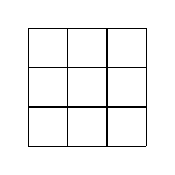
\begin{tikzpicture}[scale=0.5]
            \draw (0,0) grid (3,3);
        \end{tikzpicture}
    \end{center}

    \begin{block}{Solution}
        $(3 + 2 + 1) \times (3 + 2 + 1) = \mathbf{36}$.
    \end{block}
\end{frame}

\begin{frame}
    \frametitle{Grading}

    The grade will be based on:
    \begin{itemize}
        \item homework (45\%),
        \item quizzes (15\%), and
        \item two 1.5-hour exams (20\% each).
    \end{itemize}

    This course will \underline{not} be graded on a curve, i.e., there are not a set percentage of each grade to be given out.

    Final grade cutoffs:
    \begin{itemize}
        \item total score of 90\% guarantees the final grade of A or higher;
        \item total score of 80\% guarantees the final grade of B or higher;
        \item total score of 70\% guarantees the final grade of C or higher;
        \item total score of 60\% guarantees the final grade of D.
    \end{itemize}
\end{frame}

\begin{frame}
    \frametitle{Exams and quizzes}
    \begin{block}{Exams (20\% each)}
        There will be two exams, each covering one half of the course. These exams will \underline{not} be cumulative.
    \end{block}

    \begin{block}{Quizzes (15\% total)}
        There will be three quizzes, administered via Canvas:
        \begin{itemize}
            \item at the end of next week, on Friday-Saturday, January 17-18;
            \item at the end of the week after, on Friday-Saturday, January 24-25;
            \item in the first week after spring break.
        \end{itemize}

        The goal of the first two quizzes is to help you decide whether this course is a good match for you.
    \end{block}
\end{frame}

\begin{frame}
    \frametitle{Counting permutations}
    \begin{block}{Theorem}
        An $n$-element set has $n!$ permutations.
    \end{block}

    \[
        \boxed{n=3} \quad 123 \quad 132 \quad 213 \quad 231 \quad 312 \quad 321
    \]

    \begin{block}{Proof \#1: selecting the entries, left to right}
        $n$ choices for the $1^{\text{st}}$ entry, then $n-1$ choices for the $2^{\text{nd}}$ entry, etc.
    \end{block}

    \begin{block}{Proof \#2: inserting the entries, in increasing order}
        \[
            \begin{array}{c|cccccc}
                n=3 & 123  & 132  & 213  & 231  & 312  & 321  \\
                \hline
                n=4 & 1234 & 1324 & 2134 & 2314 & 3124 & 3214 \\
                    & 1243 & 1342 & 2143 & 2341 & 3142 & 3241 \\
                    & 1423 & 1432 & 2413 & 2431 & 3412 & 3421 \\
                    & 4123 & 4132 & 4213 & 4231 & 4312 & 4321
            \end{array}
        \]
    \end{block}
\end{frame}

\begin{frame}
    \frametitle{The Addition Principle (=Summation Rule)}
    Two incarnations of the Addition Principle:
    \begin{enumerate}
        \item splitting a set into subsets;
        \item splitting choices into cases.
    \end{enumerate}

    \begin{block}{Problem}
        How many squares can be found in this picture?
    \end{block}

    \begin{center}
        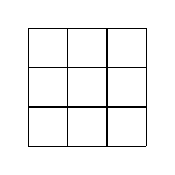
\begin{tikzpicture}[scale=0.5]
            \draw (0,0) grid (3,3);
        \end{tikzpicture}
    \end{center}

    \begin{block}{Solution}
        $16 + 9 + 4 + 1 = \mathbf{30}$.

        (We shall later solve this for the $n \times n$ grid.)
    \end{block}
\end{frame}

\begin{frame}
    \frametitle{Proofs}
    This is a \underline{proof-based} course. Students are expected to understand rigorous mathematical proofs, and perhaps even more importantly, supply their own proofs when asked.

    Some specific prerequisites:
    \begin{itemize}
        \item proofs by induction,
        \item proofs by contradiction,
        \item basic set theory terminology (intersection, union, etc.),
        \item basic function terminology (one-to-one, onto, composition, etc.).
    \end{itemize}

    If you are not familiar with Mathematical Induction, read either [Bóna, Chapter 2] or [Shahriari, Sections 1.1-1.2].
\end{frame}

\begin{frame}
    \frametitle{Content overview}
    This course introduces the fundamental notions, techniques, and theorems of \textit{enumerative combinatorics} and \textit{graph theory}.

    Level: undergraduate. Next level courses: Math 565, Math 566.

    Recommended texts (neither is required):
    \begin{itemize}
        \item M. Bóna, \textit{A walk through combinatorics}, $4^{\text{th}}$ ed., World Scientific, 2016-17.
        \item S. Shahriari, \textit{Invitation to Combinatorics}, Cambridge University Press, 2022.
    \end{itemize}

    We will roughly cover Part II (\textit{Enumerative Combinatorics}) and Part III (\textit{Graph Theory}) of Bóna's textbook, plus some other topics.

    We will not follow either textbook too closely. The lectures and the books will often provide slightly different approaches.
\end{frame}

\begin{frame}
    \frametitle{The golden rule}

    \begin{block}{The golden rule of counting}
        Count everything \underline{exactly} once.
    \end{block}

    That is: count everything, and don't count anything more than once.

    As we develop more sophisticated methods of counting, it will be important to make mental checks that everything is accounted for, and nothing is overcounted.
\end{frame}

\begin{frame}
    \frametitle{Unordered set partitions}
    \begin{block}{Problem}
        In how many ways can a 4-element set be partitioned into nonempty subsets (=blocks)?

        Example: distributing students among Zoom breakout rooms.
    \end{block}

    \begin{block}{Solution}
        There are 4 cases, depending on the number of blocks:
        \begin{itemize}
            \item 1 block: $abcd$
            \item 2 blocks: $abc | d \quad abd | c \quad acd | b \quad bcd | a \quad ab | cd \quad ac | bd \quad ad | bc$
            \item 3 blocks: $ab | c | d \quad ac | b | d \quad ad | b | c \quad bc | a | d \quad bd | a | c \quad cd | a | b$
            \item 4 blocks: $a | b | c | d$
        \end{itemize}
        Total: $1 + 7 + 6 + 1 = 15$.

        Exercise: Solve the analogous problem for a 5-element set.
    \end{block}
\end{frame}

\begin{frame}
    \frametitle{Homework}
    There will be approximately 11 problem sets, posted on Canvas.

    Homework \#1 will be released on Tuesday, Jan 14. It will be due on Jan 20 at 11:59pm.

    Homework \underline{answers have to be justified}. No justification---no credit.

    Collaboration in small groups (up to four people total in a group) is allowed---but each case of collaboration has to be explicitly acknowledged on every homework submission.
\end{frame}

\begin{frame}
    \frametitle{Homework submission and grading}
    Homework submission and grading will be done via Gradescope.

    On each problem set, only 5 problems will be graded.

    Late homework will \underline{not} be accepted.

    The lowest homework score will be dropped in the final calculation.

    Gradescope has a built-in mechanism for regrade requests.

    Any questions about the administrative aspects of the course?
\end{frame}

\begin{frame}
    \frametitle{The Multiplication Principle (=Product Rule)}

    \begin{block}{Problem}
        Jimmy John's \textit{Slim Roast Beef Sandwich} can be ordered:
        \begin{itemize}
            \item on French bread, wheat bread, or without bread;
            \item with regular, extra, or small amount of roast beef;
            \item with regular, extra, small, or no amount of avocado spread;
            \item with regular, extra, small, or no amount of provolone cheese;
            \item with, without, or with extra Dijon mustard;
            \item with or without tomato.
        \end{itemize}
        How many ways are there to order the \textit{Slim Roast Beef Sandwich}?
    \end{block}

    \begin{block}{Solution}
        $3 \cdot 3 \cdot 4 \cdot 4 \cdot 3 \cdot 2 = 864$.
    \end{block}
\end{frame}

\end{document}